\documentclass[kdmile,a4paper]{kdmile}

\usepackage[utf8]{inputenc}
\usepackage[T1]{fontenc}
\usepackage[brazilian]{babel}
\usepackage{amsmath}
\usepackage{amssymb}
\usepackage{booktabs}
\usepackage{array}
\usepackage{graphicx,url}
\graphicspath{{figures/}}

% Permite empacotar mais floats por página, reduzindo lacunas em branco
\renewcommand{\topfraction}{0.92}
\renewcommand{\bottomfraction}{0.85}
\renewcommand{\textfraction}{0.06}
\renewcommand{\floatpagefraction}{0.75}
\setcounter{topnumber}{3}
\setcounter{bottomnumber}{2}
\setcounter{totalnumber}{5}

\newtheorem{theorem}{Theorem}[section]
\newtheorem{conjecture}[theorem]{Conjecture}
\newtheorem{corollary}[theorem]{Corollary}
\newtheorem{proposition}[theorem]{Proposition}
\newtheorem{lemma}[theorem]{Lemma}
\newdef{definition}[theorem]{Definition}
\newdef{remark}[theorem]{Remark}

\markboth{J. Teixeira and C. Caminha}
{Garbage Bag Identification and Localization}
\title{Specialized Detection or Zero-Shot Vision-Language Modeling? Garbage Bag Identification and Localization in Brazilian Street Images}

\author{Jaime Teixeira, Carlos Caminha}

\institute{Kunumi Lab - Universidade Federal do Ceará (UFC), Fortaleza, CE, Brasil\\
\email{jaimejrs@alu.ufc.br, caminha@ufc.br}}


\begin{abstract}
Monitoring garbage bags on public roads requires large-scale inspection under limited operational resources. This study compares YOLOv11m, fine-tuned as a specialized detector, and Gemma 4 31B-QAT, used as a zero-shot vision-language model, for identifying the presence and location of garbage bags in Brazilian street images. YOLOv11m was fine-tuned on 4,235 positive images from two Roboflow garbage-bag datasets and 424 negative roadway scenes. Both models were evaluated on a balanced external test set of 560 Google Street View screenshots from multiple Brazilian states, annotated and cross-reviewed by two researchers. Gemma achieved higher F1-score for binary identification (0.9650 versus 0.8685), while YOLOv11m achieved substantially higher per-image localization success at intersection over union (IoU) 0.5 (0.8071 versus 0.3821) and higher box-level F1-score (0.5744 versus 0.1546). YOLOv11m processed approximately 98 images per second end-to-end, whereas Gemma's average latency was approximately 126 times higher. These results reveal a complementary accuracy--latency--localization trade-off. A cascade in which Gemma confirms presence before YOLO localizes reduced false positives by 36.0\% and raised the box-level F1 to 0.5942, at the cost of lower recall, indicating that hybrid pipelines can balance precision and coverage.
\end{abstract}

\begin{CCSXML}
<ccs2012>
<concept>
<concept_id>10010147.10010257.10010258.10010259</concept_id>
<concept_desc>Computing methodologies~Object detection</concept_desc>
<concept_significance>500</concept_significance>
</concept>
<concept>
<concept_id>10010147.10010257.10010282</concept_id>
<concept_desc>Computing methodologies~Computer vision</concept_desc>
<concept_significance>500</concept_significance>
</concept>
<concept>
<concept_id>10010405.10010469.10010474</concept_id>
<concept_desc>Applied computing~Environmental sciences</concept_desc>
<concept_significance>300</concept_significance>
</concept>
</ccs2012>
\end{CCSXML}
\ccsdesc[500]{Computing methodologies~Object detection}
\ccsdesc[500]{Computing methodologies~Computer vision}
\ccsdesc[300]{Applied computing~Environmental sciences}

\keywords{garbage bag detection, object detection, public administration, vision-language models, YOLOv11m}

\begin{document}

\begin{bottomstuff}
Os autores gostariam de agradecer à FUNCAP (Fundação Cearense de Apoio ao Desenvolvimento Científico e Tecnológico) e ao Instituto Kunumi pela infraestrutura computacional disponibilizada e pelo apoio à realização desta pesquisa.
\end{bottomstuff}

\maketitle

\section{Introdução}
\label{sec:introducao}

A gestão de resíduos sólidos urbanos envolve impactos ambientais, sanitários, financeiros e operacionais. No Brasil, a Política Nacional de Resíduos Sólidos atribui aos municípios papel central na organização da coleta e destinação dos resíduos \cite{Brasil2010}, cujos custos dependem diretamente da estrutura operacional adotada \cite{Rodrigues2016}.

A produção de informações territorializadas sobre o descarte irregular de sacos de lixo pode apoiar a priorização de áreas, o planejamento de rotas e a fiscalização. Entretanto, a inspeção manual de grandes volumes de imagens demanda tempo e recursos humanos. Técnicas de visão computacional oferecem a possibilidade de transformar registros visuais de ruas em alertas administrativos, mas sua utilidade depende não apenas da acurácia, como também da velocidade, da ocorrência de falsos alarmes, da rastreabilidade e da infraestrutura necessária para operação.

Detectores da família YOLO localizam rapidamente instâncias e retornam caixas que facilitam a auditoria \cite{Redmon2016YOLO,Ultralytics2024YOLO11}. Modelos de visão e linguagem (VLMs) associam imagens e instruções e podem operar em regime \emph{zero-shot}, sem ajuste no conjunto-alvo \cite{Radford2021CLIP}. Essa flexibilidade reduz o treinamento inicial, mas pode elevar o custo de inferência.

Estudos anteriores mostraram que a análise automatizada de resíduos enfrenta dificuldades associadas a materiais deformáveis, sobrepostos, parcialmente oclusos e inseridos em cenas visualmente carregadas \cite{Bashkirova2022ZeroWaste,Abid2025WasteDetection}. Paralelamente, a supervisão conjunta de imagens e linguagem possibilitou classificação visual \emph{zero-shot} \cite{Radford2021CLIP} e métodos de detecção aberta que combinam conhecimento semântico e localização \cite{Kuo2023FVLM,Jin2024FineGrainedDescriptors}. Comparações entre detectores supervisionados e VLMs fundacionais devem considerar a assimetria do pré-treinamento e o alinhamento dos conceitos aprendidos ao domínio-alvo \cite{Madan2024FewShotVLM}. Apesar desses avanços, a literatura revisada oferece evidência limitada sobre a comparação direta, nas mesmas imagens brasileiras de vias públicas, entre um detector especializado e um grande modelo visão-linguagem para identificar a presença e determinar a localização de sacos de lixo, considerando também o custo de inferência.

Este trabalho investiga as seguintes perguntas de pesquisa:
\begin{itemize}
    \setlength{\itemsep}{0pt}
    \setlength{\parsep}{0pt}
    \setlength{\topsep}{2pt}
    \item \textbf{RQ1:} Como se comparam um detector especializado com \emph{fine-tuning} e um VLM generalista em \emph{zero-shot} na identificação da presença e na localização de sacos de lixo em imagens reais de vias públicas brasileiras?
    \item \textbf{RQ2:} Qual é o trade-off entre desempenho na identificação e localização de sacos de lixo, eficiência computacional e adequação aos diferentes cenários de monitoramento urbano?
\end{itemize}

As principais contribuições são: uma comparação controlada, em imagens brasileiras de vias públicas, entre um detector especializado e um VLM generativo, considerando a identificação da presença de sacos de lixo, sua localização espacial e a eficiência computacional; a análise pareada da identificação binária e da localização dos sacos por caixas delimitadoras; e a caracterização dos cenários em que cada paradigma apresenta maior viabilidade operacional.

O restante deste trabalho está organizado como segue: a Seção~\ref{sec:trabalhos-relacionados} revisa trabalhos relacionados; a Seção~\ref{sec:metodologia} descreve a metodologia; a Seção~\ref{sec:resultados} apresenta os resultados e a discussão; e a Seção~\ref{sec:conclusao} conclui o trabalho.

\section{Trabalhos Relacionados}
\label{sec:trabalhos-relacionados}

\subsection{Detecção automatizada de sacos de lixo}
\label{sec:deteccao-residuos}

A detecção de objetos busca identificar e localizar instâncias por meio de caixas delimitadoras. Detectores de uma etapa, como o YOLO, realizam a predição conjunta de classes e regiões, favorecendo aplicações de baixa latência \cite{Redmon2016YOLO,Ultralytics2024YOLO11}, em contraste com detectores de duas etapas baseados em propostas de região. A avaliação desses métodos consolidou-se em torno do critério $\mathrm{IoU} \ge 0{,}5$ do PASCAL VOC \cite{Everingham2010VOC} e da precisão média (AP) calculada sobre múltiplos limiares de IoU no COCO \cite{Lin2014COCO}, convenções adotadas também neste trabalho.

No domínio de resíduos, aplicações urbanas como o SpotGarbage empregaram redes convolucionais profundas para detectar regiões com lixo em imagens capturadas por smartphones \cite{Mittal2016SpotGarbage}. O conjunto ZeroWaste, por sua vez, evidenciou que a segmentação de resíduos deformáveis, sobrepostos, oclusos e em fundos visualmente carregados permanece um problema difícil, com AP de segmentação baixo mesmo para fortes \emph{baselines} supervisionados \cite{Bashkirova2022ZeroWaste}. Avaliações recentes também demonstraram que deslocamento de domínio e formulação linguística afetam o desempenho de métodos supervisionados e de vocabulário aberto \cite{Abid2025WasteDetection}. Embora esses trabalhos cubram resíduos heterogêneos, este estudo adota um recorte mais estrito: apenas sacos usados para acondicionar lixo constituem o objeto-alvo, excluindo resíduos avulsos. Em nosso teste brasileiro, o detector ajustado atinge F1 de caixas de 0,5744 e sucesso por imagem de 0,8071 sob $\mathrm{IoU} \ge 0{,}5$, contextualizando a dificuldade da localização precisa nesse domínio.

\subsection{Modelos de visão e linguagem}
\label{sec:modelos-visao-linguagem}

VLMs aprendem representações conjuntas de imagens e textos. O CLIP demonstrou a transferência desse conhecimento para classificação \emph{zero-shot}, alcançando 76,2\% de acerto \emph{top-1} no ImageNet sem treinamento específico \cite{Radford2021CLIP}; o paradigma foi combinado a componentes de detecção em abordagens de vocabulário aberto \cite{Kuo2023FVLM}. Detectores fundamentados em linguagem evoluíram rapidamente: o GLIP atingiu cerca de 49,8 AP em transferência \emph{zero-shot} para o COCO \cite{Li2022GLIP}, o Grounding DINO elevou esse patamar para aproximadamente 52,5 AP \cite{Liu2024GroundingDINO} e o OWL-ViT estendeu a detecção de vocabulário aberto a \emph{Vision Transformers} \cite{Minderer2022OWLViT}. Descrições detalhadas podem melhorar o alinhamento entre conceitos e regiões \cite{Jin2024FineGrainedDescriptors}, enquanto VLMs generativos tratam tarefas visuais por instruções e saídas estruturadas \cite{Wang2023VisionLLM}.

Cabe notar que esses detectores de vocabulário aberto recebem supervisão de caixas ou \emph{grounding} durante o pré-treinamento, ao passo que avaliamos o Gemma como VLM puramente generativo, produzindo decisões binárias e coordenadas apenas por instruções. Reconhecimento global e localização fina não são problemas equivalentes; métodos híbridos combinam VLMs com componentes especializados para reduzir essa diferença \cite{Lin2024VLSAM}. Essa distinção se materializa em nossos resultados: o Gemma identifica a presença de sacos com F1 de 0,9650, mas sua localização por caixas atinge apenas F1 de 0,1546, enquanto o YOLOv11m, ajustado ao domínio, inverte essa relação.

O modelo multimodal foi carregado pelo identificador \texttt{google/gemma-4-31b-qat} do catálogo do LM Studio, baseado no repositório GGUF \path{lmstudio-community/gemma-4-31B-it-QAT-GGUF} \cite{LMStudioGemma431BQAT}. Trata-se de uma variante de 31B parâmetros com quantização ciente do treinamento (\emph{quantization-aware training}, QAT), capaz de receber imagem e texto.

\section{Metodologia}
\label{sec:metodologia}

\subsection{Tarefa e dados}
\label{sec:tarefa-dados}

A avaliação considerou duas camadas. Na primeira, cada imagem foi classificada como \textbf{com saco de lixo visível} ou \textbf{sem saco de lixo visível}. Na segunda, as caixas previstas foram comparadas às 785 caixas anotadas no teste. Para o YOLOv11m, \emph{black\_bag} e \emph{white\_bag} foram selecionadas de \emph{garbage-8uzha} (v4) \cite{roboflow2026a}, e \emph{trash bag}, de \emph{garbage-mvzg3} (v1) \cite{roboflow2026b}; todas foram agregadas na classe ``saco de lixo''. Como negativos, foram usadas 424 imagens da classe \emph{Roadway} da base Sidewalk \cite{sidewalk2022dataset} sem sacos anotados, equivalentes a 10\% das positivas. A composição é apresentada na Tabela~\ref{tab:conjuntos}.

\begin{table}[t]
\centering
\footnotesize
\caption{Composição das fontes de dados experimentais}
\label{tab:conjuntos}
\begin{tabular}{lccc}
\toprule
\textbf{Conjunto} & \textbf{Total de Imagens} & \textbf{Positivas (com saco)} & \textbf{Negativas (sem saco)} \\
\midrule
\emph{garbage-8uzha} (v4) & 3.370 & 3.370 & 0 \\
\emph{garbage-mvzg3} (v1) & 865 & 865 & 0 \\
\emph{Roadway} (fundo) & 424 & 0 & 424 \\
Teste brasileiro & 560 & 280 & 280 \\
\bottomrule
\end{tabular}
\end{table}

O teste foi construído com capturas do Google Street View \cite{google2026policy} de diferentes estados brasileiros, sem sobreposição com o treinamento. Dois pesquisadores anotaram o conjunto de forma independente: cada um anotou 50\% das imagens e revisou os 50\% restantes, com divergências ajustadas por consenso; todos os sacos visíveis foram delimitados individualmente. O conjunto é balanceado (280 positivas e 280 negativas), tratando resíduos avulsos, vegetação e objetos utilitários como negativos.

A integridade das divisões foi verificada por deduplicação perceptual com \emph{pHash} (distância máxima de 5), agrupando variações da mesma imagem e impedindo correspondências entre treino e teste. Rostos e placas foram anonimizados ou recortados quando na margem da imagem.

\subsection{Modelos e configurações}
\label{sec:modelos-configuracoes}

O experimento comparou duas estratégias de adoção --- treinar um modelo especializado ou empregar um generalista sem treinamento adicional ---, detalhadas na Tabela~\ref{tab:configuracao}.

\begin{table}[t]
\centering
\footnotesize
\caption{Configuração dos modelos experimentais}
\label{tab:configuracao}
\begin{tabular}{lp{4.2cm}p{5.2cm}}
\toprule
\textbf{Configuração} & \textbf{YOLOv11m} & \textbf{Gemma 4 31B-QAT} \\
\midrule
Regime & \emph{Fine-tuning} supervisionado & \emph{Zero-shot} \\
Saída principal & Caixas, confiança e classe por imagem & Classe binária e caixas em JSON \\
Identificador/pesos & \emph{yolo11m.pt} & \texttt{google/gemma-4-31b-qat} \\
Quantização de execução & Não aplicável & GGUF Q4\_0 \\
Épocas & 100 & Não aplicável \\
Resolução & 640 $\times$ 640 & Imagem original processada pelo servidor \\
\emph{Batch size} & 12 & Inferência individual \\
Otimizador & AdamW & Não aplicável \\
Taxa de aprendizado inicial & 0,001 & Não aplicável \\
\emph{Early stopping} & Paciência 20 & Não aplicável \\
\emph{Augmentation} & \emph{mosaic=1.0}, \emph{fliplr=0.5} & Não aplicável \\
Limiar principal & 0,25 & Resposta binária; caixas sem confiança \\
Temperatura & Não aplicável & 0 \\
\emph{Seed} & 42 & 42 \\
\bottomrule
\end{tabular}
\end{table}

O melhor \emph{checkpoint} do YOLO foi selecionado via validação ($\ge 0{,}25$). O Gemma 4 31B-QAT corresponde ao identificador \texttt{google/gemma-4-31b-qat} executado no LM Studio 0.4.15 a partir do arquivo GGUF \path{gemma-4-31B-it-QAT-Q4_0.gguf} (quantização Q4\_0, 18,85~GB).\footnote{Dois prompts solicitaram, respectivamente, a presença de ao menos um saco e a localização individual de até 20 sacos. Os textos estão em \texttt{prompt\_gemma\_classificacao.txt} e \texttt{prompt\_gemma\_localizacao.txt}, com hashes SHA-256 registrados nos artefatos de cada execução.}

As caixas do Gemma foram normalizadas em 0--1000 e os resíduos avulsos, excluídos. Um parser robusto isola o JSON por captura de chaves (\emph{brackets matching}) e o valida com \emph{jsonschema}; em falha de parsing ou timeout, a imagem seria conservadoramente rotulada como negativa, embora as 560 respostas tenham sido estruturadas com sucesso.

\subsection{Avaliação}
\label{sec:avaliacao}

Para a identificação binária, foram calculadas acurácia, precisão, sensibilidade, especificidade, F1-score (Equação~\ref{eq:f1}), taxa de falsos positivos, kappa de Cohen, coeficiente de correlação de Matthews e matrizes de confusão. Para a localização, caixas previstas e anotadas foram pareadas por interseção sobre união (\emph{Intersection over Union}, IoU, Equação~\ref{eq:iou}) com limiar $\mathrm{IoU} \ge 0{,}5$, reportando precisão, \emph{recall} e F1 por caixas, sucesso em imagens positivas e melhor IoU médio por imagem.
\begin{equation}
\mathrm{IoU}(A,B) = \frac{|A \cap B|}{|A \cup B|}
\label{eq:iou}
\end{equation}
\begin{equation}
\mathrm{F1} = \frac{2 \cdot \mathrm{TP}}{2 \cdot \mathrm{TP} + \mathrm{FP} + \mathrm{FN}}
\label{eq:f1}
\end{equation}
\noindent onde $A$ e $B$ são as áreas da caixa prevista e da caixa anotada; TP, FP e FN são contados com limiar IoU $\ge 0{,}5$. O mAP não foi comparado porque o Gemma retornou caixas sem confiança ranqueável.

Intervalos de confiança de 95\% foram estimados pelo método de Wilson e as discordâncias avaliadas pelo teste de McNemar. A latência e o \emph{throughput} foram medidos em uma GPU RTX 5090. No YOLO, o tempo incluiu a leitura local e inferência; no Gemma, o tempo decorrido entre a requisição HTTP e a resposta.

\section{Resultados e Discussão}
\label{sec:resultados}

\subsection{Desempenho na identificação e localização}
\label{sec:desempenho-preditivo}

A Tabela~\ref{tab:desempenho} apresenta as métricas obtidas no conjunto de 560 imagens, separando a identificação binária por imagem da localização por caixas.

\begin{table}[t]
\centering
\scriptsize
\setlength{\tabcolsep}{4pt}
\renewcommand{\arraystretch}{0.95}
\caption{Desempenho na identificação e localização de sacos de lixo}
\label{tab:desempenho}
\begin{tabular}{lccc}
\toprule
\textbf{Métrica} & \textbf{YOLOv11m} & \textbf{Gemma 4 31B-QAT} & \textbf{Diferença} \\
\midrule
\multicolumn{4}{l}{\textit{Identificação binária por imagem}} \\
Acurácia & 0,8643 & \textbf{0,9661} & +0,1018 \\
Precisão & 0,8423 & \textbf{0,9962} & +0,1539 \\
Sensibilidade & 0,8964 & \textbf{0,9357} & +0,0393 \\
Especificidade & 0,8321 & \textbf{0,9964} & +0,1643 \\
F1-score & 0,8685 & \textbf{0,9650} & +0,0965 \\
Taxa de falsos positivos & 0,1679 & \textbf{0,0036} & $-0,1643$ \\
\addlinespace[2pt]
\multicolumn{4}{l}{\textit{Localização por caixas (IoU $\ge 0,5$)}} \\
TP/FP/FN caixas & 388/178/397 & 127/731/658 & $-261$/+553/+261 \\
F1-score caixas & \textbf{0,5744} & 0,1546 & $-0,4198$ \\
Sucesso em imagens positivas & \textbf{0,8071} & 0,3821 & $-0,4250$ \\
IoU médio da melhor caixa & \textbf{0,6894} & 0,4278 & $-0,2616$ \\
\bottomrule
\end{tabular}
\end{table}

Na identificação binária, o Gemma apresentou vantagem em todas as métricas, com diferença mais expressiva na precisão (1 falso positivo contra 47 do YOLO) e especificidade (0,9964 contra 0,8321).

Na localização, o padrão inverteu-se: das 785 caixas anotadas, o YOLO pareou 388 com $\mathrm{IoU} \ge 0,5$ contra 127 do Gemma, que gerou 858 caixas previstas. A vantagem do YOLO foi altamente significativa ($p \approx 5{,}8 \times 10^{-27}$ para sucesso por imagem), consistente com a distinção entre reconhecimento global e localização regional \cite{Lin2024VLSAM}. A Figura~\ref{fig:iou-dist} evidencia essa separação. Assim, em resposta à \textbf{RQ1}, o Gemma supera na identificação binária e o YOLO na localização espacial.

\begin{figure}[t]
\centering
\IfFileExists{figures/fig_distribuicao_iou_localizacao.png}{%
  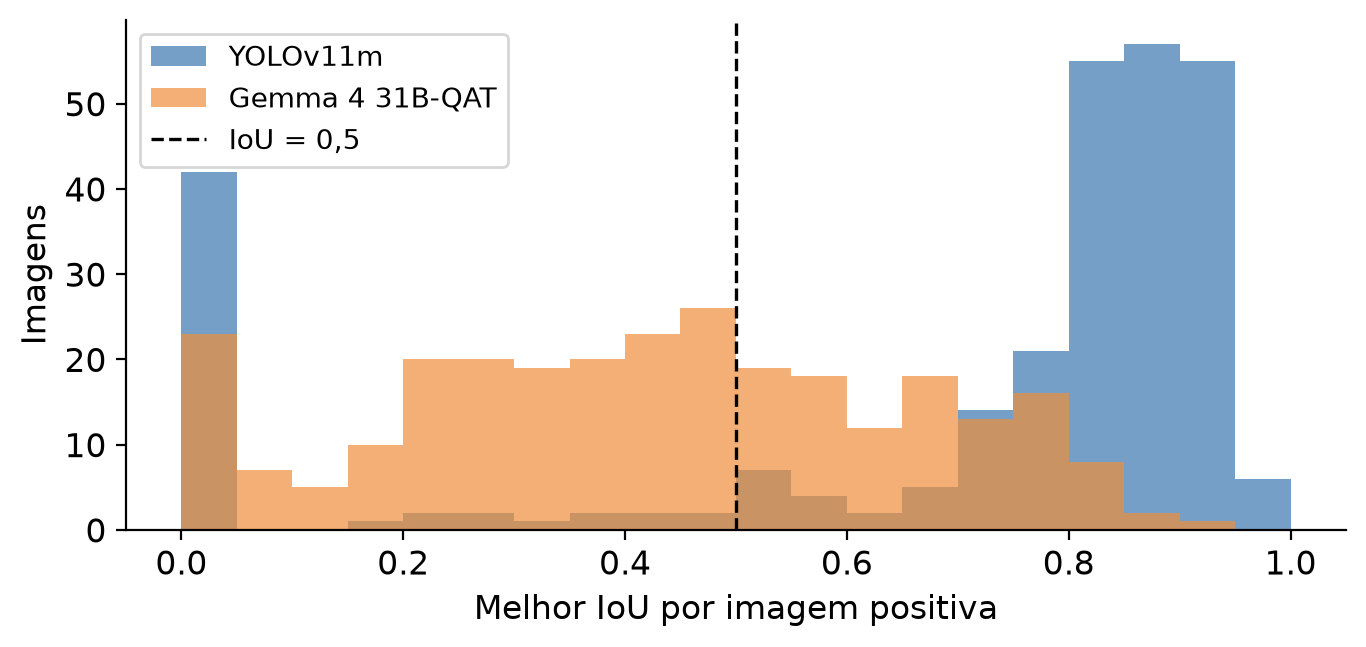
\includegraphics[width=0.72\linewidth]{figures/fig_distribuicao_iou_localizacao.png}%
}{%
  \IfFileExists{../outputs/figures/fig_distribuicao_iou_localizacao.png}{%
    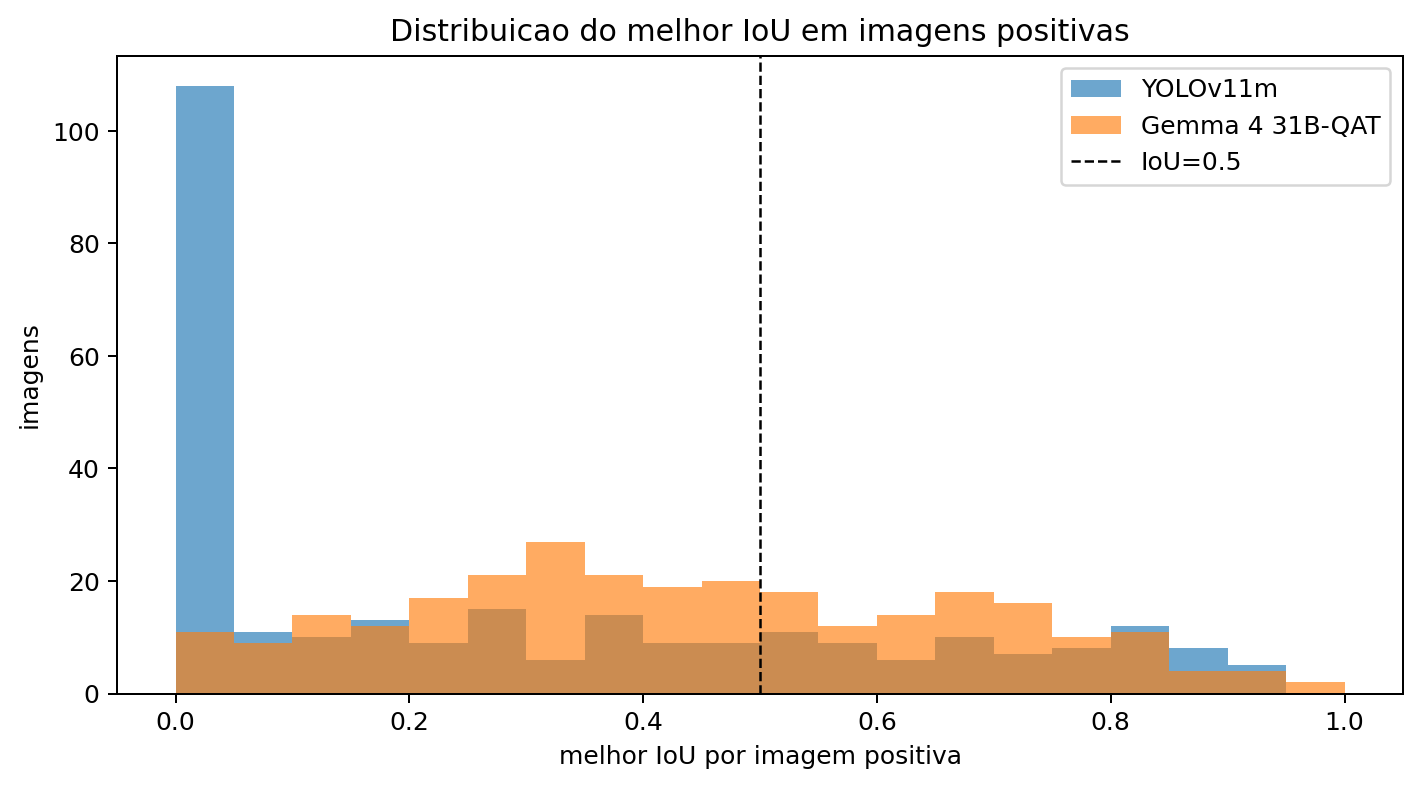
\includegraphics[width=0.72\linewidth]{../outputs/figures/fig_distribuicao_iou_localizacao.png}%
  }{%
    \fbox{\parbox{0.90\linewidth}{\centering Figura não encontrada. Execute o notebook para gerar o PNG.}}%
  }%
}
\caption{Distribuição do melhor IoU por imagem positiva ($n = 280$). O YOLO concentra-se acima de 0,5; o Gemma, abaixo.}
\label{fig:iou-dist}
\end{figure}

Os intervalos de confiança de 95\% da acurácia foram 0,833--0,890 (YOLO) e 0,948--0,978 (Gemma), e o teste de McNemar confirmou a diferença ($p \approx 3,5 \times 10^{-11}$).


\subsection{Sensibilidade ao limiar do YOLO}
\label{sec:sensibilidade-limiar}

O limiar de confiança altera o equilíbrio entre sensibilidade e falsos positivos. A Tabela~\ref{tab:limiar_yolo} apresenta os quatro pontos de operação avaliados para o YOLOv11m.

\begin{table}[t]
\centering
\footnotesize
\caption{Sensibilidade ao limiar de confiança do YOLOv11m}
\label{tab:limiar_yolo}
\begin{tabular}{lcccccc}
\toprule
\textbf{Limiar} & \textbf{Acurácia} & \textbf{Precisão} & \textbf{Sensibilidade} & \textbf{Especificidade} & \textbf{F1-score} & \textbf{FPR} \\
\midrule
0,25 & 0,8643 & 0,8423 & \textbf{0,8964} & 0,8321 & \textbf{0,8685} & 0,1679 \\
0,35 & \textbf{0,8661} & 0,8755 & 0,8536 & 0,8786 & 0,8644 & 0,1214 \\
0,50 & 0,8482 & 0,8947 & 0,7893 & 0,9071 & 0,8387 & 0,0929 \\
0,65 & 0,8268 & \textbf{0,9256} & 0,7107 & \textbf{0,9429} & 0,8040 & \textbf{0,0571} \\
\bottomrule
\end{tabular}
\par\smallskip\raggedright
\scriptsize Nota: FPR = Taxa de Falsos Positivos (\emph{False Positive Rate}).
\end{table}

O aumento do limiar reduz falsos positivos, mas eleva omissões: em 0,65, a especificidade atinge 0,9429 e a sensibilidade cai para 0,7107. O ponto de operação deve refletir o custo relativo dos erros na aplicação.

\subsection{Eficiência computacional}
\label{sec:eficiencia-computacional}

O YOLOv11m operou com latência média de 10,2~ms (98,5~imagens/s), enquanto o Gemma exigiu 1.278,6~ms (0,782~imagem/s) --- aproximadamente 126 vezes maior \cite{Madan2024FewShotVLM,Magalhaes2019EdgeCloudYOLO}. Em resposta à \textbf{RQ2}, o Gemma oferece melhor identificação binária, enquanto o YOLO apresenta menor latência, maior throughput e localização superior.

\subsection{Análise dos erros e complementaridade}
\label{sec:analise-erros}

Os modelos discordaram em 79 imagens (68 acertadas só pelo Gemma, 11 só pelo YOLO). Na localização, o YOLO acertou 130 imagens não localizadas pelo Gemma, contra 11 no sentido oposto; os falsos positivos do VLM concentraram-se em contêineres e sacolas (Figura~\ref{fig:caixas-tp-fp-fn}) \cite{Kuo2023FVLM,Lin2024VLSAM}.

\begin{figure}[t]
\centering
\IfFileExists{figures/fig_amostras_localizacao_fp_fn.png}{%
  \includegraphics[width=0.98\linewidth]{figures/fig_amostras_localizacao_fp_fn.png}%
}{%
  \IfFileExists{../outputs/figures/fig_amostras_localizacao_fp_fn.png}{%
    \includegraphics[width=0.98\linewidth]{../outputs/figures/fig_amostras_localizacao_fp_fn.png}%
  }{%
    \fbox{\parbox{0.90\linewidth}{\centering Figura não encontrada. Execute o notebook para gerar o PNG.}}%
  }%
}
\caption{Localização no teste: verde = referência, vermelho = YOLO, azul = Gemma. O YOLO alinha-se ao \emph{ground truth}; o Gemma gera caixas em excesso. \copyright~2026 Google, uso acadêmico, elementos sensíveis anonimizados.}
\label{fig:caixas-tp-fp-fn}
\end{figure}

Esses resultados motivaram uma cascata em que o Gemma confirma a presença (limiar binário) e o YOLO localiza apenas as imagens positivas. Das 280 imagens positivas, a cascata obteve sucesso em 219 (0,7821), com TP/FP/FN de caixas = 380/114/405, precisão = 0,7692, recall = 0,4841 e F1 = 0,5942. Comparada ao YOLO isolado (sucesso 0,8071, 178~FP, F1 = 0,5744), a cascata reduziu os falsos positivos em 36,0\% e elevou o F1 de caixas, ao custo de menor cobertura --- os falsos negativos do Gemma propagam-se pela cascata, reduzindo o recall.

\subsection{Implicações para a gestão pública}
\label{sec:implicacoes-gestao}

Os resultados sugerem três usos principais: o YOLOv11m em monitoramento contínuo, pela baixa latência e localização precisa; o Gemma 4 31B-QAT em auditorias pontuais orientadas à identificação binária, pela alta precisão e baixa taxa de falsos positivos; e a cascata Gemma $\to$ YOLO quando a redução de falsos positivos justifica a perda de cobertura. Em todos os cenários, a adoção deve incluir revisão humana, auditoria de decisões e reavaliação periódica.

\section{Conclusão}
\label{sec:conclusao}

Este trabalho comparou YOLOv11m e Gemma 4 31B-QAT na identificação e localização de sacos de lixo em 560 imagens de vias públicas brasileiras. O Gemma obteve melhor desempenho na identificação binária (F1 = 0,9650 versus 0,8685), enquanto o YOLOv11m demonstrou localização substancialmente superior (taxa de sucesso 0,8071 versus 0,3821 e F1 de caixas 0,5744 versus 0,1546), sendo aproximadamente 126 vezes mais rápido. Uma cascata Gemma $\to$ YOLO reduziu falsos positivos em 36,0\% e elevou o F1 de caixas para 0,5942, ao custo de menor cobertura.

Os resultados não sustentam a adoção universal de um único modelo: o Gemma favorece cenários orientados à qualidade preditiva na identificação, enquanto o YOLO é mais apropriado a triagens em larga escala e à localização precisa de instâncias. Trabalhos futuros devem avaliar o desempenho sob prevalência natural (não balanceada), medir a latência completa da cascata em cenários de produção, ampliar a base municipal e testar modelos VLM menores.

\noindent\textbf{Limitações.} A amostra é balanceada artificialmente (50\% positivas), diferindo da prevalência real. A tarefa restringe-se à presença visual de sacos, sem estimar volume ou risco sanitário. A anotação por consenso entre dois pesquisadores não produz medida independente de concordância interanotador. As medições de eficiência representam os fluxos implementados (Gemma via HTTP/LM Studio, YOLO local), sem experimentos de energia ou custo em produção \cite{Madan2024FewShotVLM}.

\noindent\textbf{Disponibilidade de código e dados.} Os artefatos de reprodução e o notebook estão disponíveis em \url{https://github.com/jaimejrs/garbage-bag-yolov11m-vs-gemma4}. As imagens do Google Street View foram utilizadas exclusivamente para avaliação, com anonimização dos elementos sensíveis, respeito aos termos de uso aplicáveis e sem redistribuição não autorizada.

\bibliographystyle{kdmile}
\bibliography{garbage-bag-yolov11m-vs-gemma4}

\begin{received}
\end{received}

\end{document}
